\section{TX-Path Transfer Function}
ToDo Text (Variable Gain with Vdd of RA60, XY V for every gain)

\subsection{TF of RA60H1317M1A}
	\begin{figure}[ht!]
		\centering
		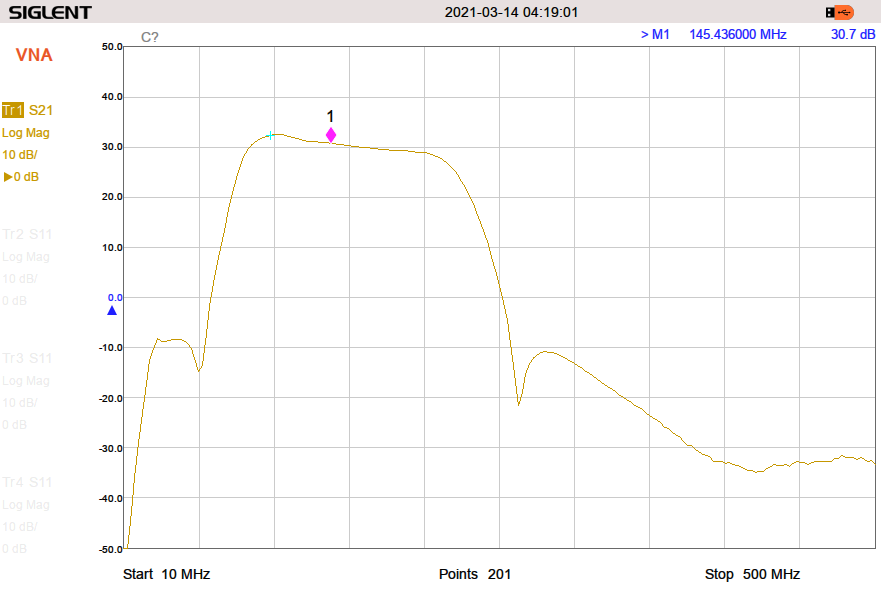
\includegraphics[width = 12cm]{./5_measurements/fig/RA60H-TF}
		\caption{Transfer Function of RA60H1317M1A}
		\label{fig:ra60h1317m1a TF}
	\end{figure}
	\newpage

\subsection{10dB Gain}
\begin{figure}[ht!]
	\centering
	\includegraphics[width = 12cm]{example-image}
	\caption{TX-Path Transfer Function with 10dB gain}
	\label{fig:10dB Gain}
\end{figure}

\subsection{30dB Gain}
	\begin{figure}[ht!]
		\centering
		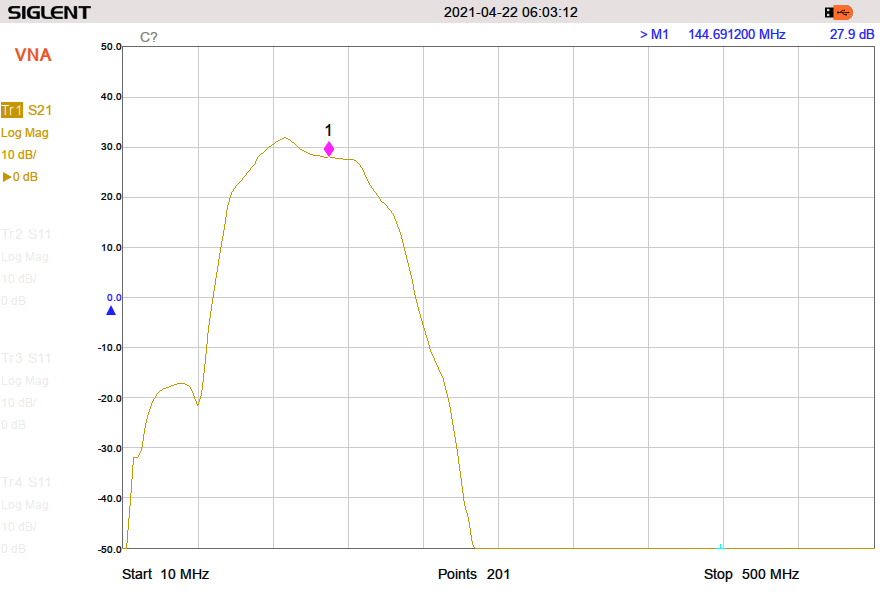
\includegraphics[width = 12cm]{./5_measurements/fig/TX-Path}
		\caption{TX-Path Transfer Function with 30dB gain}
		\label{fig:30dB Gain}
	\end{figure}
	\newpage
	
\section{RX-Path Transfer Function}
ToDo Text (Variable Attenuation with F2255)

\subsection{F2255NLGK Attenuation Diagram}
ToDo Text (What is a F2255)

	\begin{figure}[ht!]
		\centering
		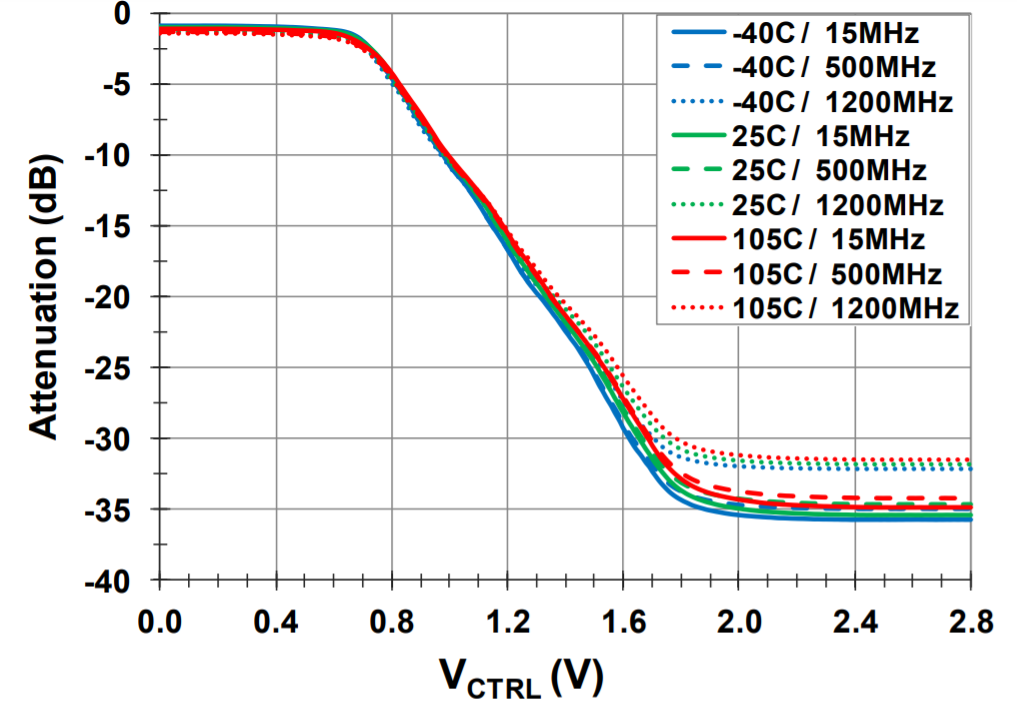
\includegraphics[width = 12cm]{./5_measurements/fig/F2255-Diagram}
		\caption{F2255NLGK Attenuation Diagram\protect\footnotemark \cite{f2255nlgk.2020}}
		\label{fig:F2255NLGK Att}
	\end{figure}

	\footnotetext{\url{https://www.mouser.at/datasheet/2/698/IDT_F2255_Datasheet_DST_20180209-1997542.pdf}}
	\newpage

\subsection{No Attenuation}
	\begin{figure}[ht!]
		\centering
		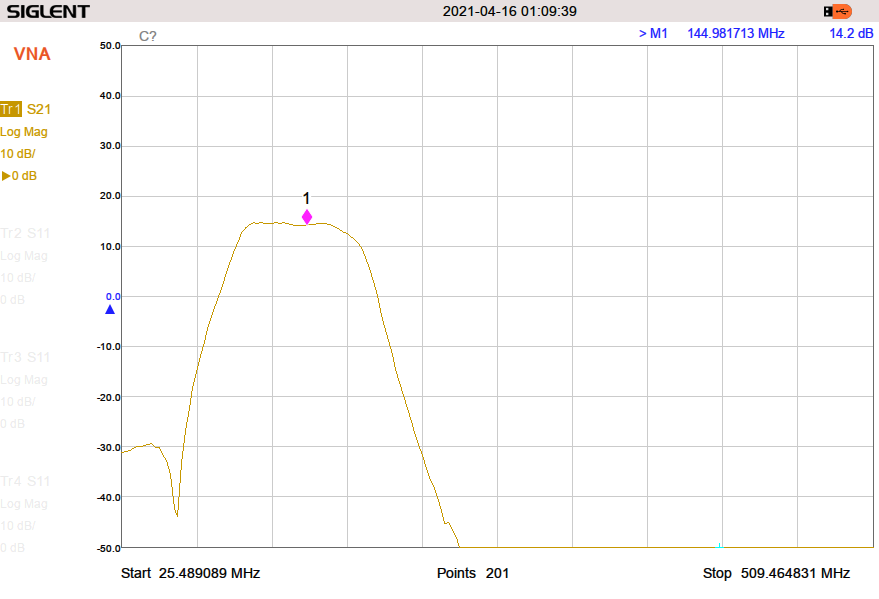
\includegraphics[width = 12cm]{./5_measurements/fig/RX-Path-NoAtt}
		\caption{RX-Path Transfer Function without attenuation}
		\label{fig:No Att}
	\end{figure}

\subsection{20dB Attenuation}
	\begin{figure}[ht!]
		\centering
		\includegraphics[width = 12cm]{example-image}
		\caption{RX-Path Transfer Function with 20dB attenuation}
		\label{fig:20dB Att}
	\end{figure}
	\newpage
	
\section{Output Power}
For all output power measurements an input power of XYdBm (xyW) is used.
Furthermore, at the input of the Vector Network Analyzer a 23dBm attenuator is mounted to handle the power.
So, the final output Power consists of the measured power and the 23dBm.\\
For exmaple, if the spectrum analyser shows an output power of XYdBm the output power equals $XY+23dBm = dBm (XYW)$.

\subsection{20W Output Power} 
	\begin{figure}[ht!]
		\centering
		\includegraphics[width = 12cm]{example-image}
		\caption{20W Output Power}
		\label{fig:20W OUT}
	\end{figure}
	\newpage

\subsection{40W Output Power}
	\begin{figure}[ht!]
		\centering
		\includegraphics[width = 12cm]{example-image}
		\caption{40W Output Power}
		\label{fig:40W OUT}
	\end{figure}

\subsection{60W Output Power}
	\begin{figure}[ht!]
		\centering
		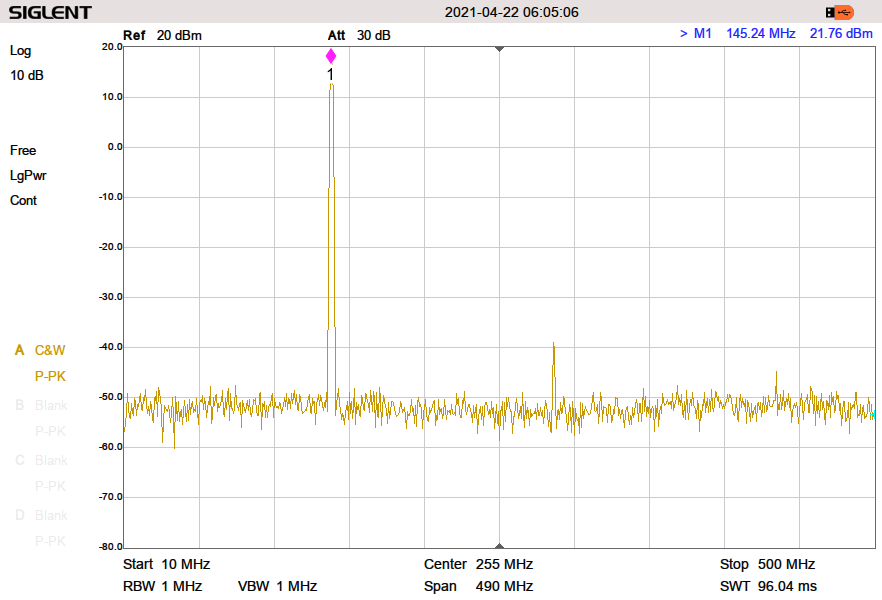
\includegraphics[width = 12cm]{./5_measurements/fig/60W-Out}
		\caption{60W Output Power}
		\label{fig:60W OUT}
	\end{figure}